% CoRL 2026 Workshop "Do Robots Need World Models? A Debate on Dynamics Learning, Planning, and
% End-to-End Robot Learning" (https://do-robots-need-world-models.github.io) -- DRAFT v1 (2026-10-03)
% Research-paper track. Up to 4 pages, CoRL template. Submit on OpenReview:
% https://openreview.net/group?id=robot-learning.org/CoRL/2026/Workshop/do-robots-need-world-models
% Deadline 2026-10-12; notification 10-26; camera-ready 11-06; workshop 11-12. Reciprocal review: one
% author must review another submission. Archival: TBD. Not double-blind as far as the page says;
% kept anonymous to be safe. References assumed outside the 4 pages (CoRL convention): check.
% Build: cd paper && tectonic -X compile main.tex  (corl_2026.sty, corlabbrvnat.bst: official kit).
\documentclass{article}
\usepackage{corl_2026}             % official CoRL 2026 submission style (anonymous); [final] for camera-ready
\usepackage[T1]{fontenc}           % Times (ptm) under XeTeX/Tectonic; harmless under pdfLaTeX
\usepackage{booktabs,amsmath,amssymb,graphicx,xcolor,tikz}
\usetikzlibrary{positioning,arrows.meta}
\definecolor{inkc}{HTML}{1B2430}\definecolor{mutedc}{HTML}{5D6873}\definecolor{linec}{HTML}{C3CAD1}
\definecolor{cardc}{HTML}{F2F4F6}\definecolor{tealc}{HTML}{0E7A86}\definecolor{orangec}{HTML}{C96A14}
\definecolor{violetc}{HTML}{6B55C9}
\newcommand{\todo}[1]{\textcolor{red}{[TODO: #1]}}

\title{Accurate on Average, Blind at the Fork}
\author{Anonymous Authors}

\begin{document}
\maketitle

\begin{abstract}
Before a robot executes an action, it should know whether its own uncertainty could change the outcome.
People make this judgment with an intuitive physics engine \citep{battaglia2013simulation}: they run a
few noisy simulations over an uncertain scene and call it precarious when the outcomes disagree. We
build this check for robots as a goal-free \emph{fork probe}: sample the robot's measured perception and
execution error, roll the intended action chunk forward 64 times, and flag it when the futures split.
With a physics engine and a real camera-based perception model, the probe catches 88\% of forks on
unseen layouts with 7\% false alarms, reading outcomes from images alone. Without the engine the probe needs a world model, and there it fails: a
token-space world model that predicts 3--4$\times$ better than a no-motion baseline catches only 18\%,
because its sampled uncertainty has the right size but not where futures branch; five further generative
variants catch at most 3\%, while sampling perception uncertainty into the start and simulating
deterministically reaches 69\%, a ceiling that more data, frame history and a DINO-WM transformer
do not lift. Safe deployment needs world models with \emph{branching fidelity}, which average-error
benchmarks do not measure.
\end{abstract}

\keywords{World models, intuitive physics, uncertainty, safe deployment}

\section{Introduction}
Manipulation policies, from diffusion policies to vision-language-action models, act by committing to
short action chunks \citep{chi2023diffusion,zhao2023act,black2024pi0}. Deploying them safely requires a
check before each chunk runs. Existing monitors address \emph{epistemic} uncertainty, flagging inputs the
model has not seen \citep{seo2025uncertainty,xu2025failure}. We address a second kind that remains even
for a perfect model: \emph{physical} uncertainty. When a robot picks a block standing between two
others, the same command can lift it cleanly or tip a neighbour depending on millimetres of execution error and
perception error. Such a chunk is risky even if its nominal outcome is fine: whether it succeeds depends on errors the
robot cannot control.

People handle this with an \emph{intuitive physics engine} (IPE): a few approximate simulations over an
uncertain scene, whose disagreement signals precariousness
\citep{battaglia2013simulation,smith2013sources,sanborn2013reconciling}. Our goal is to give robots the
same ability, which needs two things: an honest model of the robot's own uncertainty, and a model to
simulate with. Outside simulation the second must be learned, which gives the physical fidelity of world
models a concrete, safety-relevant test: a world model is useful here only if its rollouts branch where
the real dynamics branch, a property prediction error does not measure.

\paragraph{Contributions.} (1) A \emph{fork probe}: a pre-execution check that propagates the robot's
measured perception and execution uncertainty through a rollout engine and flags splits, with no task
labels, failure data or fitted thresholds (Sec.~\ref{sec:probe}). (2) Validation with a physics engine and
real camera perception on three unseen test sets, which sets the reference a world model must reach
(Sec.~\ref{sec:validation}). (3) \emph{Branching fidelity} as a world-model evaluation, and two learned
token-space world models that predict well on average yet fail it, with a diagnosis (Sec.~\ref{sec:wm}).

\section{Setup and the fork probe}\label{sec:probe}
\paragraph{Task.} Three Jenga-like blocks stand upright in a row; a simulated Franka Panda (MuJoCo) must
pick the middle (red) block without toppling its neighbours. At each chunk start a policy commits to an 8-step action chunk; ours come from recorded episodes, but the probe treats
the policy as a black box and sees only the chunk, one camera image and proprioception.

\paragraph{Fragility.} A chunk is \emph{fragile} if the robot's uncertainty, its execution error and its
error in perceiving the scene, can send the outcome into qualitatively different regimes. This needs no
goal or failure label, which a monitor around a generalist policy cannot assume, and it isolates exactly
the cases where intent no longer determines the outcome. For our task we measure it physically: a state
is a \emph{fork} if some but not all of 64 futures sampled from this uncertainty (2--62) topple a
neighbouring block. A chunk that fails every time is not a fork and needs a task-level check.

\paragraph{Uncertainty model.} Execution error comes from the robot's measured tracking residuals
(median chunk maximum 3.2\,mm). Perception is a frozen DINOv2 encoder \citep{oquab2024dinov2} on one
close-camera image with a keypoint head for the three blocks in play (2.5\,mm held-out error); its error
model is measured once, offline, as a zero-mean Gaussian fitted to its errors on held-out images with
known poses (a full $9\times9$ position covariance capturing correlated errors, plus rotation covariances).

\paragraph{Fork probe and rollout engine} (Fig.~\ref{fig:forks}a). The probe imagines 64 versions of the
chunk. Each starts from the perceived scene shifted by one sampled perception error and runs the chunk
with one sampled execution error; a 30-step imagined hold then lets the outcome settle. It flags
the chunk if, at hold steps 10 and 30, the endings (object positions or image tokens) projected on their
first principal axis prefer two Gaussians to one by BIC, are well separated (Ashman's $D>2$
\citep{ashman1994detecting}), have at least 2 members in the smaller group, and keep the same grouping;
these are fixed statistical conventions, not fitted to labels. A variant draws 5 scene hypotheses and
flags if at least 3 split. The probe works with any rollout engine. Our reference is MuJoCo with the
three blocks placed at the sampled poses and everything else (block geometry, masses, friction) taken from
the simulator, which a real robot does not have; the learned alternative is a world model (Sec.~\ref{sec:wm}).

\paragraph{Ground truth.} One real outcome cannot grade a monitor, since a fragile chunk may succeed by
luck. An oracle therefore samples the 64 futures from the \emph{true} scene in exact physics and labels
the state a fork as above. Two independent oracle runs give the same label on 99\% of states. Every evaluation uses unseen block layouts (about 60 screened forks plus 100
safe states) under a protocol frozen before the data existed.

\section{Results}
\subsection{Propagating uncertainty through a physics engine works}\label{sec:validation}
On the 112 states used to design the split test (exact physics, true scene), it flags all 23 topple
forks and 10\% of the 89 states without one. With real perception, perception uncertainty must be
propagated: errors of 2--4\,mm are comparable to execution noise, and a probe that trusts the estimate
catches only 65--67\% of forks, while the fork probe catches 77--91\% with 7--17\% false alarms
(Table~\ref{tab:panels}). Reading outcomes from DINOv2 tokens of rendered endings instead of object
positions costs almost nothing, so the probe works from images alone: on test set C it catches 88\%
of forks (95\% CI 77--94\%) with 7\% false alarms. This is the reference a world model must reach.

\begin{figure}[t]
\centering
% Figure 1 (a): the fork probe as a pipeline. Images: exact replays of held-out state ep63_seed104_s74
% (paper/render_fork_frames.py). Ghost images average the 64 imagined starts / endings.
\begin{tikzpicture}[
  font=\footnotesize, every node/.append style={execute at begin node={\hyphenpenalty=10000\relax}},
  stage/.style={font=\scriptsize\bfseries\color{inkc}, anchor=south},
  note/.style={font=\scriptsize, text=mutedc, align=center, anchor=north, text width=2.3cm},
  img/.style={inner sep=0pt, draw=linec, line width=0.4pt},
  card/.style={draw=linec, fill=cardc, rounded corners=3pt, line width=0.4pt, align=center,
               minimum height=2.15cm, inner sep=3pt, font=\scriptsize},
  flow/.style={-{Stealth[length=4pt]}, line width=0.7pt, draw=mutedc},
]
\def\w{2.15cm}
% 1 camera image
\node[img] (cam) at (0,0) {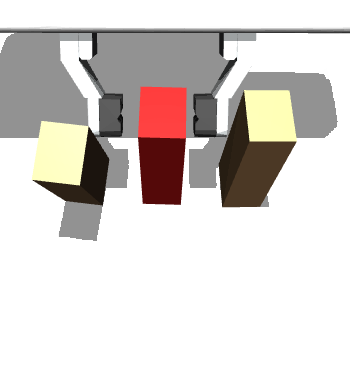
\includegraphics[width=\w]{fig_assets/crop_start.png}};
\node[stage] at (cam.north) {camera image};
\node[font=\small\bfseries, anchor=south east] at ([xshift=-2pt,yshift=10pt]cam.north west) {(a)};
\node[note] at (cam.south) {perceived block poses\\(2.5\,mm error)};
% 2 the robot's uncertainty
\node[img, right=0.55cm of cam] (unc) {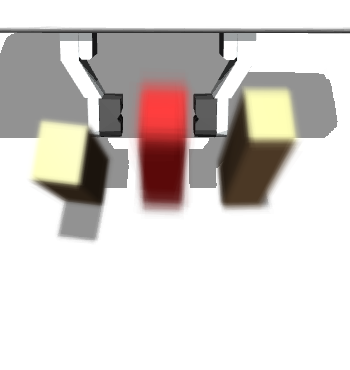
\includegraphics[width=\w]{fig_assets/crop_start_ghost.png}};
\node[stage] at (unc.north) {\textcolor{tealc}{its own uncertainty}};
\node[note] at (unc.south) {64 plausible scenes (measured perception error) $\times$ measured execution error};
% 3 rollout engine
\node[card, right=0.55cm of unc, text width=2.15cm] (eng) {%
  \textbf{rollout engine}\\[3pt]
  8-step chunk\\then 30-step\\imagined hold\\[4pt]
  \textcolor{inkc}{MuJoCo}\\{\color{mutedc}(reference)}\\[1pt] or\\[1pt]
  \textcolor{violetc}{learned world model}};
% 4 imagined futures
\node[img, right=0.55cm of eng] (fut) {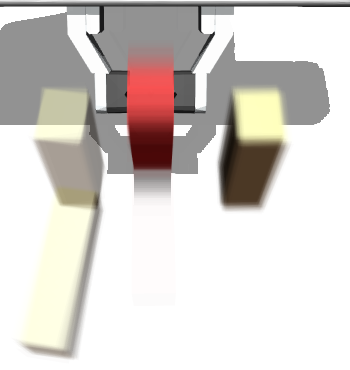
\includegraphics[width=\w]{fig_assets/crop_end_ghost.png}};
\node[stage] at (fut.north) {\textcolor{orangec}{64 imagined futures}};
\node[note] at (fut.south) {the neighbour stays (31)\\or topples (33)};
% 5 decision
\node[card, right=0.55cm of fut, text width=1.9cm] (dec) {%
  \textbf{split test}\\[3pt]
  two persistent,\\well-separated\\groups?\\[4pt]
  \textcolor{orangec}{\textbf{yes: fragile}}\\[1pt]
  {\color{mutedc}slow down,\\re-perceive, replan}};
\draw[flow] (cam.east) -- (unc.west);
\draw[flow] (unc.east) -- (eng.west);
\draw[flow] (eng.east) -- (fut.west);
\draw[flow] (fut.east) -- (dec.west);
\end{tikzpicture}
\\[4pt]
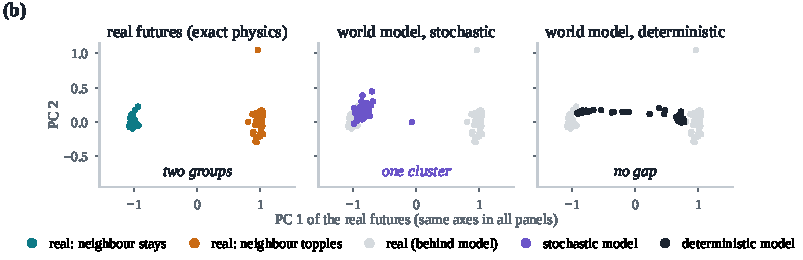
\includegraphics[width=0.96\linewidth]{fig_futures.pdf}
\caption{(a) The fork probe on one held-out state (exact renders; images average all 64 samples).
(b) The same 64 futures in the world model's latent space, on the real futures' principal axes.}
\label{fig:forks}
\end{figure}

\begin{table}[t]
\centering
\caption{Fork probe (MuJoCo, real perception) on unseen test sets: forks caught / false alarms (\%).}
\label{tab:panels}
\small
\begin{tabular}{lcccccc}
\toprule
& \multicolumn{2}{c}{Set A (153 states)} & \multicolumn{2}{c}{Set B (160)} & \multicolumn{2}{c}{Set C (156)} \\
outcomes read from object positions & caught & false & caught & false & caught & false \\
\midrule
perception uncertainty ignored & 65 & 23 & 65 & 12 & 67 & 24 \\
fork probe & 90 & 12 & 77 & 8 & 91 & 10 \\
fork probe, 5 hypotheses & 90 & 17 & 90 & 13 & 89 & 11 \\
\midrule
outcomes read from images: fork probe & 88 & 12 & 77 & 8 & 88 & 9 \\
\phantom{outcomes read from images:} 5 hypotheses & -- & -- & -- & -- & \textbf{88} & \textbf{7} \\
\bottomrule
\end{tabular}
\end{table}

\subsection{Propagating uncertainty through learned world models fails}\label{sec:wm}
Without privileged geometry a learned model must take MuJoCo's role, and the probe becomes its test:
given one image and the 64 perturbed chunks, do its rollouts branch where physics branches? Our
model compresses DINOv2 tokens by a fixed per-patch PCA to a $28\times28\times8$ latent (on held-out real
futures the split test on this latent catches 97\% of forks) and predicts
the next latent from the current one and the action with a flow-matching transition, drawing fresh noise
at every step. It is trained on 8 futures per image whose start scenes were sampled within the measured
perception error, so its target spread is the robot's own uncertainty; a deterministic version of the
same network is the control. Both beat a no-motion baseline on 19-step latent error by 3--4$\times$, yet
on test set C the stochastic model catches 18\% of forks and the deterministic one 60\%, against 88\% for
the engine (Table~\ref{tab:wm}).

\begin{table}[t]
\centering
\caption{World models on test set C; spread diagnostics on held-out states with 64 real futures each.}
\label{tab:wm}
\small
\begin{tabular}{lccccc}
\toprule
rollouts from & caught & false & spread & main axis & fork ratio \\
\midrule
reference (MuJoCo; real futures) & 88\% & 7\% & 1.00 & 0.57 & 4.8 \\
token world model, stochastic & 18\% & 2\% & 0.98 & 0.15 & 1.3 \\
token world model, deterministic & 60\% & 10\% & 0.04 & 0.69 & 32 \\
5 generative variants (Sec.~\ref{sec:wm}) & 0--3\%$^\dagger$ & 0--1\%$^\dagger$ & 1.1--1.6 & 0.07--0.10 & -- \\
uncertain starts + deterministic, 4$\times$ forks & 69\%$^\dagger$ & 8\%$^\dagger$ & 0.35 & 0.48 & -- \\
\bottomrule
\multicolumn{6}{l}{\footnotesize $^\dagger$ on 160 held-out training-domain states (75 forks), not set C; none passed the gate to run on a fresh set.}
\end{tabular}
\end{table}

\paragraph{Where the uncertainty went wrong.} Compared with real futures (Table~\ref{tab:wm}: total spread,
share on the main axis, ratio on forks vs other states), the stochastic model has the right \emph{amount} of uncertainty but not its \emph{shape} or \emph{placement}:
the spread is isotropic and nearly the same on forks and non-forks, the average uncertainty of futures
rather than where they branch (Fig.~\ref{fig:forks}b). (Per-step noise suits high-dimensional uncertainty, as in weather \citep{price2025gencast}.) The deterministic model's tiny spread is aligned with the branch axis and 32$\times$ larger on
forks, suggesting, as in the IPE, that uncertainty should enter through the initial conditions. In a
pre-registered factorial on 160 held-out states, generative models producing whole clips, with an
energy-score loss, 4$\times$ more fork data or an action-sensitivity loss catch 0--3\% of forks, equally isotropic. Putting the
uncertainty into the initial conditions works instead: a learned operator perturbs the start latent by
sampled perception error and deterministic dynamics roll it out, catching 52\% of forks at 7\% false
alarms, and 69\% at 8\% with 4$\times$ more fork data. Giving a generative model the same perturbed starts
does not help (0\%): noise in the learned dynamics erases forks. The deterministic recipe plateaus at
68--72\% with 3$\times$ training, more fork data, frame history or DINO-WM's predictor \citep{zhou2025dinowm}.

\section{Related work}
\paragraph{Simulation under uncertainty.} Beyond the IPE \citep{zhou2023mental}, robotics runs Monte Carlo rollouts over pose, friction or model parameters to
score grasps and pushes \citep{mahler2017dexnet,agboh2018pushing} or to build safety filters
\citep{johansson2025safety,wang2026manidreams}. \citet{cannizzaro2024cobra} sample measured perception
and placement noise through a simulator to predict whether a block tower stands, and
\citet{goyal2026stability} measure offline how fast perturbed chunks diverge. These
score a task predicate, labels \citep{lerer2016learning} or a growth rate. Closest in spirit,
\citet{zapolsky2016particle} sample model and sensor parameters to find divergent particle traces when
validating robot plans offline; they propose detecting divergence without a goal but, in their
experiments, detect it through task failure or by inspection. Our probe instead runs before every chunk,
samples the robot's own measured execution and perception errors, and applies an automatic test for
whether the outcomes split, a Monte Carlo test of proximity to a basin boundary \citep{menck2013basin}.
\paragraph{Uncertainty-aware monitors.} Latent safety filters (also on Jenga) and failure detectors use
failure classifiers, epistemic or policy uncertainty \citep{nakamura2025generalizing,seo2025uncertainty,xu2025failure,agia2024unpacking}:
what a model does not know, not whether the physics is at a branch.
\paragraph{World models and their uncertainty.} Learned simulators and latent world models
\citep{sanchezgonzalez2020learning,allen2023fignet,zhou2025dinowm,assran2025vjepa2,hafner2025dreamerv3}
struggle with stiff contact \citep{parmar2021fundamental}; audits find weak physical grounding
\citep{bear2021physion,motamed2026physicsiq,yang2026mirabench}.
\citet{yu2026evaluated} propose evaluating world models on interventional action branches, by
prediction error and action-effect agreement per branch; our models predict individual futures well yet
lose the forks, so a test of branching is needed alongside. Stochastic and ensemble models
\citep{chua2018pets,lakshminarayanan2017ensembles} are evaluated by likelihood, calibration or return,
none of which checks whether their spread splits where the dynamics branch.

\section{Conclusion and limitations}
A robot can judge fragility as people do, by propagating its own measured uncertainty through a rough
simulator. For safe deployment: physical uncertainty must be propagated,
not just estimated; without a simulator this needs world models with branching fidelity, which our
generative models lack despite low average error and uncertain starts partly recover, so benchmarks
should measure it; and until learned dynamics have it, our results favour the IPE's design, learned
perception and measured uncertainty feeding an approximate physics engine whose scene (shapes, masses,
friction) must still be estimated from sensors.
\paragraph{Limitations.} Simulation, one task with three blocks; the engine probe uses the simulator's
true shapes, masses and friction; one Gaussian models perception error for all images; test sets differ in
difficulty; each world model was trained once; pretrained world models (V-JEPA 2-AC, Cosmos) are
untested; and the probe flags forks, not certain failures.

\paragraph{Use of generative AI.} Generative AI tools (Claude) assisted with code, figures, literature
search and drafting. The authors designed the study, checked all results and references, and take full
responsibility for the content.

\bibliography{references}
\end{document}
